\documentclass[conference]{IEEEtran}
\IEEEoverridecommandlockouts
\usepackage{cite}
\usepackage{amsmath,amssymb,amsfonts}
\usepackage{algorithmic}
\usepackage{graphicx}
\usepackage{textcomp}
\usepackage{xcolor}
\usepackage{placeins}
\usepackage{booktabs} % Added for professional table formatting

\def\BibTeX{{\rm B\kern-.05em{\sc i\kern-.025em b}\kern-.08em
    T\kern-.1667em\lower.7ex\hbox{E}\kern-.125emX}}

\begin{document}

\title{CROWD SIMULATION\\
{\footnotesize Simulating the Flow: Bridging Floor-Plan Images and Realistic Crowd Dynamics}
}

\makeatletter \newcommand{\linebreakand}{%
    \end {@IEEEauthorhalign}
    \hfill\mbox{}\par
    \mbox{}\hfill\begin{@IEEEauthorhalign}
}
\makeatother

\author{
    \IEEEauthorblockN{Anshul Dalvi}
    \IEEEauthorblockA{
        22BCE10799\\
        CSE, VIT Bhopal\\
        Bhopal, India\\
        anshuldalvi2022@vitbhopal.ac.in
    }
    \and
    \IEEEauthorblockN{Dev Deep Narayan}
    \IEEEauthorblockA{
        22BCE11141\\
        CSE, VIT Bhopal\\
        Bhopal, India\\
        devdeepnarayan2022@vitbhopal.ac.in
    }
    \and
    \IEEEauthorblockN{Piyush Kumar}
    \IEEEauthorblockA{
        22BCE10725\\
        CSE, VIT Bhopal\\
        Bhopal, India\\
        piyushkumar.2022@vitbhopal.ac.in
    }

    \linebreakand\IEEEauthorblockN{Pragjyotish Lahan}
    \IEEEauthorblockA{
        22BCE10407\\
        CSE, VIT Bhopal\\
        Bhopal, India\\
        pragjyotishlahan2022@vitbhopal.ac.in
    }
    \and
    \IEEEauthorblockN{Pratham Amit Singh}
    \IEEEauthorblockA{
        22BCE10959\\
        CSE, VIT Bhopal\\
        Bhopal, India\\
        prathamamitsingh2022@vitbhopal.ac.in
    }
}

\maketitle

\begin{abstract}
    Crowd simulation plays a crucial role in the design and safety evaluation of public infrastructures such as buildings, campuses, and transportation hubs. This paper proposes an agent-based crowd simulation framework that uses floor-plan images as input to realistically model pedestrian movement and evacuation behavior. The system begins with preprocessing architectural floor plans using image processing techniques to extract walkable areas, walls, and exits. A distance field is then computed over the navigable space to provide agents with global path guidance toward designated exits. Each agent follows a behavior model that combines goal-oriented movement with local collision avoidance, allowing the simulation to reproduce realistic crowd phenomena such as congestion, bottleneck formation, and smooth lane movement. The framework is implemented using commonly available computational libraries and supports real-time visualization and flexible parameter tuning. Experimental evaluations are conducted on multiple floor-plan scenarios with varying crowd densities and exit configurations. Results demonstrate that the proposed approach achieves computational efficiency while maintaining believable crowd dynamics, making it suitable for evacuation analysis, facility planning, and academic experimentation.
\end{abstract}

\begin{IEEEkeywords}
    crowd simulation, agent-based modeling, floor-plan processing, distance field, pedestrian dynamics, evacuation modeling, collision avoidance, image processing
\end{IEEEkeywords}

\section{Introduction}
Accurate simulation of pedestrian crowds is a foundational tool for designing
safe, efficient public spaces and for planning effective evacuations. Over
time, a range of modeling paradigms—force-based dynamics, velocity-obstacle
techniques, agent-based rules, and data-driven
methods~\cite{helbing2000social,van2008reciprocal,pan2016crowd} have shown that
realistic crowd behavior can be reproduced, but many of these approaches depend
on substantial calibration, bespoke data, or heavy computation. Practical users
such as architects, facility managers, and educators often only have access to
floor-plan images or scanned architectural drawings and need a transparent,
easy-to-configure tool that converts those images into actionable simulations.
Converting floor-plan imagery into reliable simulation inputs brings specific
technical challenges: extracting walkable areas and exits from noisy or
low-resolution scans, computing global guidance that respects complex geometry,
and implementing local collision-avoidance mechanism~\cite{van2008reciprocal}
that preserves emergent phenomena (lane formation, queuing, clogging) while
remaining computationally tractable at realistic crowd sizes. Evaluation must
also produce meaningful metrics—evacuation time, throughput, and density
patterns—that are directly useful for design decisions. The goal is a balanced,
image-driven pipeline that prioritizes interpretability, reproducibility, and
interactivity without sacrificing the core behaviors that make crowd simulation
valuable.

The remainder of the paper is organized as follows. Section II formalizes the
problem and states the objectives. Section III reviews related work and
positions the proposed approach. Section IV describes the system architecture,
and Section V details the methodology including floor-plan preprocessing,
distance-field computation, agent modeling, and collision avoidance. Section VI
covers implementation and parameter settings. Sections VII and VIII describe
the experimental setup and evaluation metrics, Section IX presents results and
analysis, and Sections X and XI discuss limitations and future directions.
Section XII concludes the paper; appendices provide pseudocode, parameter
tables, and additional figures.

\section{Problem Definition and Objectives}

Designers, safety engineers, and facility managers frequently need fast,
reliable answers to questions about how people will move through a space—where
congestion forms, how long an evacuation takes, and which design choices (exit
size, corridor width, signage) meaningfully change outcomes. The core problem
addressed in this work is how to turn common, image-based floor plans into
simulation-ready representations and then use those representations to produce
realistic, interpretable crowd behavior at interactive speeds. This requires a
pipeline that tolerates the noise and variety of real architectural drawings,
computes robust global navigation cues across complex geometry, and couples
those cues with a lightweight local avoidance mechanism that preserves emergent
effects such as lane formation, bottlenecking, and queuing.

Existing methods often excel in one dimension but fall short in practice:
physics-based or data-driven models can be highly realistic but demand heavy
calibration and computation; simple rule-based approaches are fast but miss
important collective phenomena; and many systems assume availability of precise
CAD data rather than the scanned floor-plan images typically available in early
design stages. There is therefore a gap for an approach that is (a)
image-driven and tolerant of imperfect inputs, (b) interpretable so
practitioners can understand and tune behavior, and (c) computationally
efficient enough for rapid scenario testing and interactive visualization.

The objectives of this study are threefold. First, develop an automated
preprocessing pipeline that converts floor-plan images into accurate walkable
maps and reliably detects exits and obstacles. Second, design a navigation
framework that combines a distance-field-based global guide with a compact
local collision-avoidance model to reproduce key crowd phenomena while
maintaining scalability. Third, deliver an implementation that is reproducible
and usable: provide parameterized experiments across varied floor plans,
quantify outcomes using evacuation time, throughput, and density metrics, and
expose visualization tools that support design decision-making. Meeting these
objectives aims to produce a practical tool that bridges academic methods and
real-world facility planning needs.

\section{Related Work / Literature Review}

Crowd simulation methods fall into a few broad families, each with different
assumptions, strengths, and weaknesses. Early and highly influential
physics-inspired models treat pedestrian motion as if driven by ``social
forces'' that push agents toward goals and away from obstacles and other
people. The Social Force Model—originally proposed by Helbing and
Molnár~\cite{helbing1995social}—remains a canonical example: it reproduces many
emergent phenomena (lane formation, oscillations at bottlenecks) with a
compact, interpretable formulation, but can require careful parameter tuning to
avoid unrealistic artifacts at high densities.

A second major class focuses on geometric/velocity-based collision-avoidance
methods. Velocity Obstacle formulations and their reciprocal variants
(RVO/ORCA)~\cite{van2008reciprocal,berg2011reciprocal} compute collision-free
velocities by reasoning in velocity space rather than by simulating forces;
these approaches are fast, produce smooth local motion, and scale well to many
agents, which makes them popular in real-time applications (games, robotics,
interactive simulators). However, pure VO/RVO methods typically handle
short-term avoidance well but do not by themselves provide higher-level route
planning or long-range behavior without additional layers.

Agent-based and rule-based systems (including cellular automata) prioritize
flexibility: individual agents can carry states, goals, and simple rules that
together yield complex crowd-level patterns. These approaches are easy to
extend with heterogeneous behaviors (groups, leader-following, different
mobility profiles) and are common in applied practice and educational tools.
Their realism depends heavily on the choice of local rules and on whether a
robust global navigation signal (e.g., a path or potential field) is provided.

More recently, data-driven and learning-based models have advanced pedestrian
trajectory prediction and, in some cases, simulation. Recurrent and deep models
such as Social-LSTM~\cite{alahi2016social} and later GAN- and attention-based
predictors learn interaction priors from trajectory datasets and can capture
subtle social norms in movement, especially in medium-density, structured
scenes. Their strengths are predictive accuracy and the ability to generalize
patterns from data, but they typically require annotated trajectory datasets,
can be opaque (hard to interpret), and may struggle to generalize to new
floor-plan geometries without retraining.

There is also a line of work that ties layout representations (floorplans,
maps) to crowd-analysis and simulation. Recent papers explore extracting
navigational structure and behavioral features directly from
floorplans~\cite{chen2018floorplan,battaglia2021path} or from collections of
floorplan images; such work is relevant for design-stage analysis because it
avoids relying on precise CAD models and instead operates on the kind of
scanned or image-based inputs practitioners actually have. Still, many
simulation systems continue to assume structured geometric input (CAD,
graph-based maps) or rely on manual preprocessing, which limits automation.

\subsection{Comparison of Approaches}

\begin{itemize}
    \item \textbf{Realism vs.\ interpretability:} Physics-based models (e.g., Social Force) are interpretable and can reproduce classic emergent effects, but parameter sensitivity reduces robustness; learning-based models can produce highly realistic trajectories where enough data exist but are less transparent.

    \item \textbf{Local avoidance vs.\ global planning:} RVO/ORCA excels at local, collision-free motion and real-time scale, but needs a global guidance layer (distance fields, waypoints, or planners) to achieve purposeful route-following in complex floor layouts.

    \item \textbf{Data requirements and practicality:} Data-driven approaches need annotated trajectories and often domain-specific retraining; image-driven pipelines that can work from floor-plan images are more practical for early-stage design but demand robust preprocessing to extract walkable areas and exits.

    \item \textbf{Computational cost and scalability:} Rule-based and RVO-style methods are commonly used where interactivity or large populations are required; deep models tend to be heavier unless used only for offline prediction or as learned components within hybrid systems.
\end{itemize}

\begin{table}[htbp]
    \centering
    \caption{Comparison of Crowd Simulation Approaches}
    \label{tab:method_comparison}
    \renewcommand{\arraystretch}{1.2}
    \begin{tabular}{p{2.2cm}p{2.1cm}p{2.1cm}}
        \toprule
        \textbf{Feature}                                         & \textbf{SFM} & \textbf{RVO / ORCA} \\
        \midrule
        Core idea                                                &
        Force-based motion using attractive and repulsive forces &
        Velocity-based collision-free motion in velocity space                                        \\
        Movement quality                                         &
        Natural, organic, emergent patterns                      &
        Smooth and efficient, sometimes robotic                                                       \\
        Collision handling                                       &
        Soft constraints; overlaps under pressure                &
        Hard constraints; zero collisions                                                             \\
        Computational cost                                       &
        High ($O(N^2)$, optimizable)                             &
        Low to medium ($O(N)$)                                                                        \\
        Typical use                                              &
        Evacuation studies, research                             &
        Games, robotics, real-time agents                                                             \\
        Main drawback                                            &
        Parameter tuning, oscillations                           &
        Symmetric or overly polite behavior                                                           \\
        \bottomrule
    \end{tabular}
\end{table}

\subsection{Limitations in the Literature}

\begin{enumerate}
    \item \textbf{Input assumptions:} Many high-fidelity simulators assume vector/CAD inputs or detailed semantic labels; less work focuses on robust, fully automated conversion from noisy scanned floor-plan images into simulation-ready maps.

    \item \textbf{Calibration challenges:} Physics-based and learning-based methods both face calibration challenges—physics models need parameter tuning to match observed flows, while learned models often fail to generalize across geometric layouts without additional training data.

    \item \textbf{Evaluation standards:} Quantitative metrics and standardized evaluation protocols for crowd simulators are still an active area of research (how to compare emergent behaviors meaningfully, how to validate against real crowds), which complicates cross-paper comparisons. Recent work has begun to propose and test richer evaluation suites.

    \item \textbf{Gap in hybrid systems:} While hybrid systems (distance-field global guidance + efficient local avoidance) are conceptually attractive, few published pipelines emphasize reproducible, image-driven workflows that are lightweight enough for interactive experiment design and that come with clear evaluation across varied floor plans.
\end{enumerate}

\subsection{How This Work Connects to Prior Art}

Building on the strengths above, the proposed framework aims to combine robust,
automated floor-plan preprocessing with a distance-field-based global navigator
and an efficient local avoidance mechanism (informed by RVO/force ideas). The
goal is a pragmatic, reproducible middle path: enough structure to capture
realistic crowd phenomena, yet simple and fast enough for interactive scenario
testing and practical use by designers who only have image-based floor plans.

\section{System Overview and Architecture}

\subsection{Overall System Design}

The system is a simple, modular pipeline that converts a floor-plan image into
a usable simulation. In three quick steps it (1) reads and cleans the floor
plan, (2) builds a lightweight navigation guide over the walkable area, and (3)
runs an agent-based simulator that uses that guide plus local avoidance to
produce movement and metrics. The design intentionally keeps modules small and
well separated so you can swap or tune one part (for example, the avoidance
rule).

\begin{itemize}
    \item \textbf{Input:} raw floor-plan image (optional metadata).
    \item \textbf{Core:} Preprocessing $\to$ Distance-field / Navigator $\to$ Simulation Core.
    \item \textbf{Output:} visualization and Metrics (images, plots, logs).
\end{itemize}

\subsection{Module Interaction}

\begin{itemize}
    \item Preprocessing --- turn image $\to$ binary walkable mask and find exits.
    \item Navigator --- compute a distance field from exit; agents query it for a desired
          heading.
    \item Simulation Core --- spawn agents, combine heading + local avoidance, step
          positions, log events.
    \item Visualization and Metrics --- render frames, compute evacuation time,
          throughput, and density maps.
\end{itemize}

\section{Methodology}

\subsection{\textbf{Floor Plan Preprocessing}}

The simulation begins with a floor-plan image that represents the layout of the
environment. Since floor plans may vary in quality, resolution, and format,
basic image preprocessing is applied to standardize the input. The image is
first converted to grayscale and then filtered to reduce noise. Thresholding
techniques are used to separate structural elements from the background,
followed by morphological operations to remove small artifacts and fill gaps.
This step ensures that walls, corridors, and open spaces are clearly
distinguishable and suitable for further processing.

\subsection{\textbf{Walkable Area Extraction}}

After preprocessing, the system identifies regions that agents are allowed to
traverse. Non-walkable elements such as walls and obstacles are removed,
leaving a binary representation of walkable space. Exits are detected as
openings connected to the boundary of the walkable region or as predefined
markers in the floor plan. The resulting walkable area mask provides a
consistent spatial representation that constrains agent motion and prevents
unrealistic behaviors such as passing through walls.

\subsection{\textbf{Distance Field Computation}}

To guide agents toward exits, a distance field is computed over the walkable
area~\cite{sethian1996fast}. Each cell in the field stores the shortest
distance to the nearest exit, considering obstacles. This distance information
creates a smooth potential surface over the environment. By following the
negative gradient of the distance field, agents obtain a global sense of
direction that naturally leads them toward exits while respecting the layout
geometry. This approach avoids explicit path planning while remaining efficient
and robust.

During navigation, agents select their preferred movement direction by
minimizing a local cost function defined as
\begin{equation}
    C(\mathbf{c}) = D(\mathbf{c}) + \lambda \rho(\mathbf{c}),
\end{equation}
where $D(\mathbf{c})$ is the precomputed distance-to-exit value at cell
$\mathbf{c}$, $\rho(\mathbf{c})$ denotes the local crowd density, and
$\lambda$ controls the influence of density-based avoidance.

\subsection{\textbf{Agent Modeling}}

Each pedestrian is modeled as an autonomous agent with simple, interpretable
properties such as position, preferred walking speed, and personal space
radius. Agents are initialized at valid spawn locations within the walkable
area and are assigned exit goals. The model assumes homogeneous agents for
simplicity, though parameters can be adjusted to introduce variation. Agent
states are updated at each simulation step based on navigation cues and
interactions with nearby agents and obstacles.

Formally, each agent $i$ is represented by the state
\begin{equation}
    \mathbf{s}_i(t) = \big(\mathbf{x}_i(t), \mathbf{v}_i(t), a_i(t)\big),
\end{equation}
where $\mathbf{x}_i(t) \in \mathbb{R}^2$ denotes the agent position,
$\mathbf{v}_i(t) \in \mathbb{R}^2$ denotes its velocity, and
$a_i(t) \in \{0,1\}$ indicates whether the agent is active (not yet exited).

\subsection{\textbf{Navigation and Collision Avoidance}}

Agent movement is determined by combining global navigation and local
interaction. The global component is derived from the distance field, which
provides a preferred direction of motion toward the exit. To prevent
collisions, a local avoidance mechanism adjusts this direction based on nearby
agents and obstacles. This combination allows agents to move purposefully while
exhibiting realistic crowd behaviors such as queuing, lane formation, and
congestion near bottlenecks.

Agent motion is governed by a weighted steering formulation. The velocity
update is expressed as
\begin{equation}
    \mathbf{v}_i(t+\Delta t) =
    \mathbf{v}_i(t) +
    \left(
    w_g(\mathbf{v}_i^* - \mathbf{v}_i)
    + \mathbf{f}_i^{\text{wall}}
    + \mathbf{f}_i^{\text{social}}
    \right)\Delta t,
\end{equation}
where $\mathbf{v}_i^*$ is the desired velocity toward the exit derived from
the distance field, $\mathbf{f}_i^{\text{wall}}$ is a wall repulsion term,
and $\mathbf{f}_i^{\text{social}}$ models inter-agent separation.

\subsection{\textbf{Simulation Workflow}}

The simulation proceeds in discrete time steps. At each step, agents query the
distance field to determine their desired direction, apply collision avoidance
adjustments, and update their positions accordingly. Boundary checks ensure
agents remain within walkable regions. Agents are removed from the simulation
once they reach an exit. Throughout the simulation, key metrics such as
evacuation time, flow rate, and local density are recorded for analysis. The
process continues until all agents have exited or a predefined termination
condition is met.

\subsection{Algorithmic Overview}

\begin{algorithmic}[1]
    \STATE Load floor-plan image and generate grid map
    \STATE Detect exits and compute distance field
    \STATE Initialize agents and spatial hash
    \WHILE{agents remain in the environment}
    \STATE Compute local density field
    \FOR{substep $=1$ to $K$}
    \STATE Predict agent motion toward exits
    \STATE Resolve inter-agent and wall collisions
    \STATE Commit updated positions
    \ENDFOR
    \STATE Update metrics and render visualization
    \ENDWHILE
\end{algorithmic}

\section{Evaluation Metrics}

The performance and realism of the proposed crowd simulation framework are
evaluated using quantitative metrics that capture evacuation efficiency, crowd
dynamics, spatial congestion patterns, and computational behavior. These
metrics are derived from agent-level trajectories and density fields and are
designed to provide interpretable insights into safety, efficiency, and layout
quality.

Evaluation of crowd simulators commonly relies on evacuation time, density, and
throughput-based
metrics~\cite{seyfried2005fundamental,hoogendoorn2004pedestrian}.

\subsection{\textbf{Formal Metric Definitions}}

The evaluation metrics are computed directly from agent trajectories and
spatiotemporal density fields generated during simulation.

\subsection{\textbf{Evacuation Progress and Time}}

Evacuation performance is evaluated by tracking the cumulative number of agents
that successfully exit the environment over time. Individual evacuation times
are recorded for each agent, and the total evacuation time is defined as the
moment when the last agent reaches an exit. Percentile-based measures such as
the 90th or 95th percentile evacuation time capture late-stage congestion
effects.

Steeper cumulative evacuation curves indicate smoother crowd flow and effective
exit utilization, while flatter tails correspond to congestion near
bottlenecks.

The total evacuation time $T_{\text{total}}$ is defined as the time at which
the last agent exits the environment. Additionally, the $t_{90}$ metric denotes
the time required for 90\% of agents to evacuate:
\begin{equation}
    t_{90} = \min \{ t \mid N_{\text{exit}}(t) \geq 0.9 N \},
\end{equation}
where $N_{\text{exit}}(t)$ is the cumulative number of exited agents and
$N$ is the total population.

\begin{figure}[htbp]
    \centering
    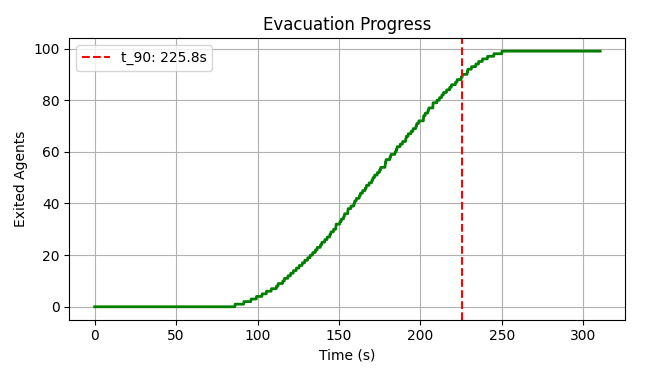
\includegraphics[width=\columnwidth]{images/exit_vs_time.png}
    \caption{Cumulative evacuation progress showing the number of agents that have exited the environment over time.}
    \label{fig:evacuation_progress}
\end{figure}

\FloatBarrier

\subsection{\textbf{Crowd Density Heatmaps}}

To analyze spatial congestion patterns, both time-averaged and peak density
heatmaps are computed. The time-averaged heatmap highlights persistent
congestion regions, while the peak congestion heatmap captures worst-case
crowding scenarios.

\begin{figure}[htbp]
    \centering
    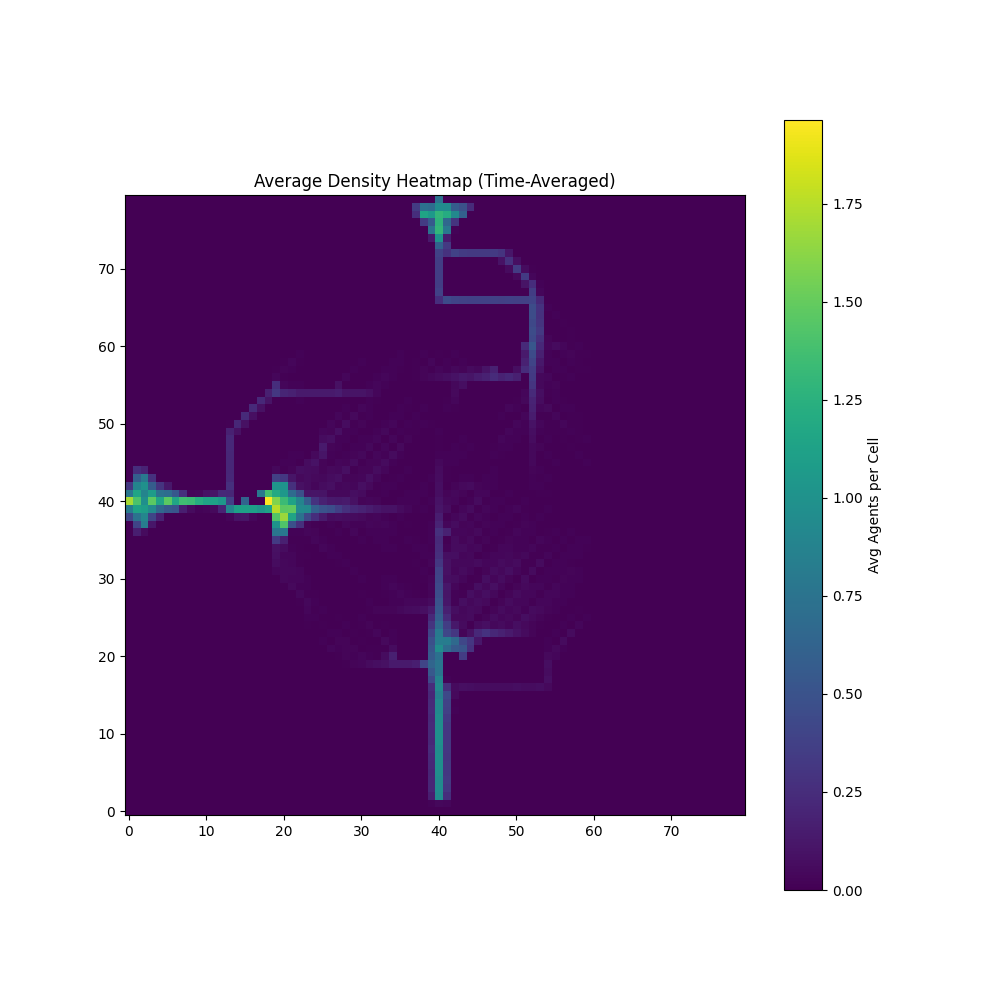
\includegraphics[width=0.48\columnwidth]{images/heatmap_average.png}
    \hfill
    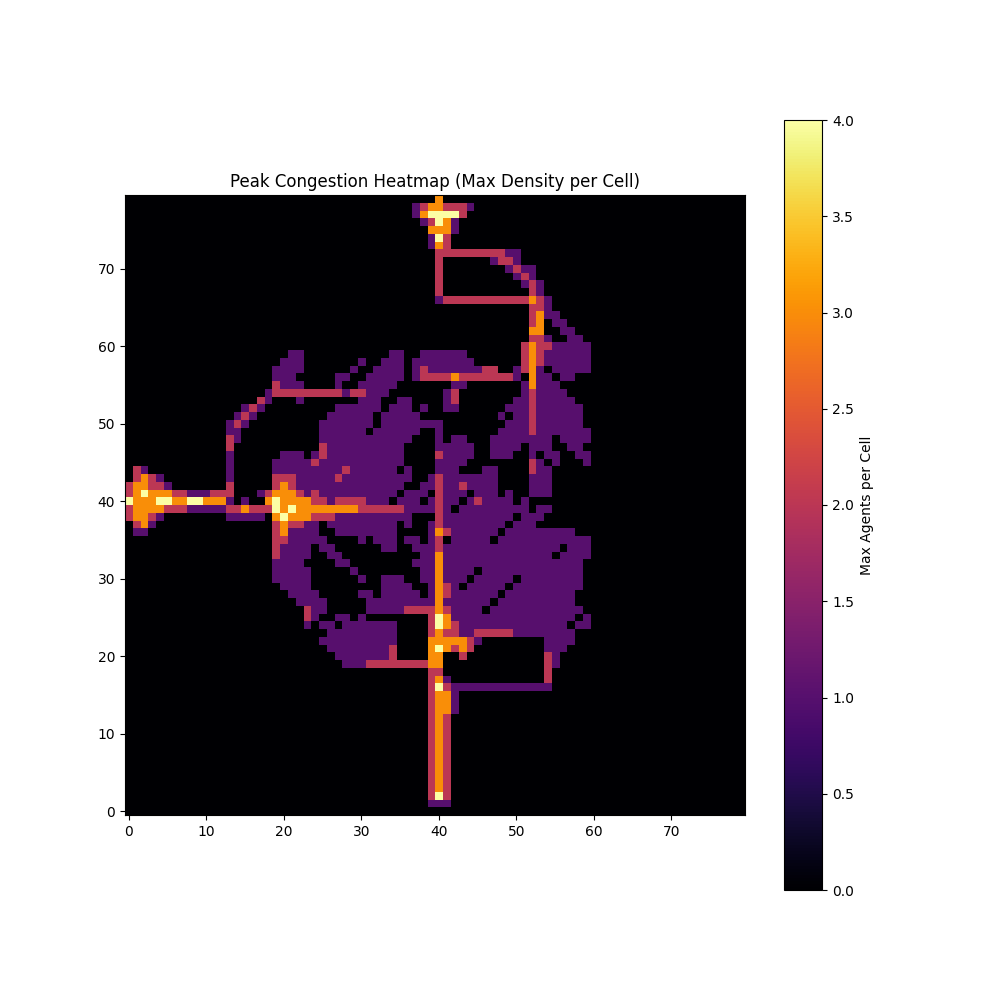
\includegraphics[width=0.48\columnwidth]{images/heatmap_peak.png}
    \caption{Spatial congestion analysis. (Left) Time-averaged crowd density showing persistent pedestrian load. (Right) Peak congestion heatmap highlighting worst-case crowding regions.}
    \label{fig:density_heatmaps}
\end{figure}

In addition to peak and average density visualization, a density overload
metric is computed to quantify sustained overcrowding. Let $\rho(\mathbf{c},
    t)$ denote the number of agents in grid cell $\mathbf{c}$ at time $t$. The
density overload ratio is defined as
\begin{equation}
    \rho_{\text{over}} =
    \frac{1}{|\mathcal{C}|T}
    \sum_{t}\sum_{\mathbf{c}}
    \mathbb{I}\big(\rho(\mathbf{c}, t) > \rho_{\text{safe}}\big),
\end{equation}
where $\mathcal{C}$ is the set of grid cells, $T$ is the number of simulation
time steps, and $\rho_{\text{safe}}$ is a predefined safety threshold.

\FloatBarrier

\subsection{\textbf{Crowd Speed}}

Crowd mobility is evaluated using average crowd speed over time. Average speed
is computed across all agents at each simulation step, providing insight into
global mobility trends. Sustained reductions in speed indicate congestion and
inter-agent interference.

Average crowd speed is computed as
\begin{equation}
    \bar{v}(t) = \frac{1}{N_a} \sum_{i \in \mathcal{A}} \|\mathbf{v}_i(t)\|,
\end{equation}
where $\mathcal{A}$ denotes the set of active agents.

\begin{figure}[htbp]
    \centering
    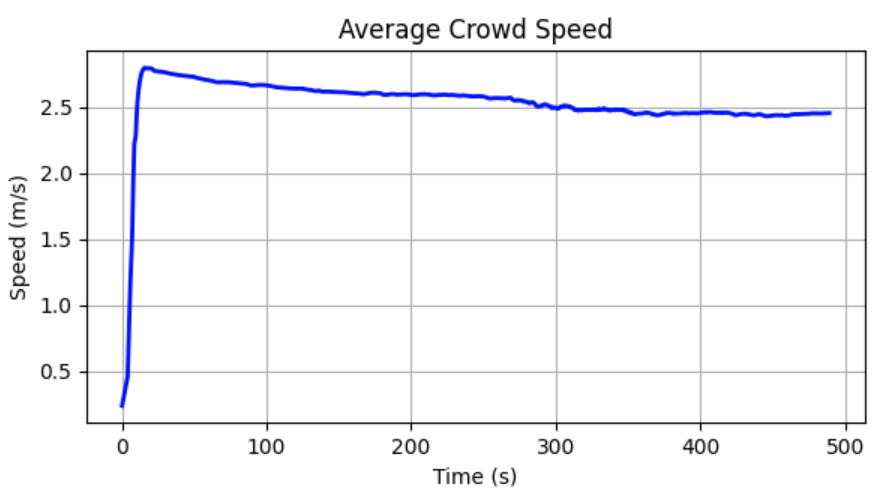
\includegraphics[width=0.8\columnwidth]{images/avg_crowd_speed.png}
    \caption{Average crowd speed over time computed across all agents.}
    \label{fig:avg_speed}
\end{figure}

\FloatBarrier

\subsection{\textbf{Collisions and Inter-Agent Distance}}

Safety and comfort are assessed through collision counts accumulated over time.
Collisions or overlaps occur when agents violate personal space constraints
during movement, typically due to high local density or limited available
space. Higher collision counts indicate increased crowd pressure, reduced
movement comfort, and a greater likelihood of unsafe interactions.

Analyzing collision trends over time helps identify critical phases of the
evacuation process when congestion intensifies, such as near exits or narrow
corridors.

A collision (or overlap) event is recorded when the distance between two agents
violates personal space constraints, defined as
\begin{equation}
    \|\mathbf{x}_i - \mathbf{x}_j\| < 2r,
\end{equation}
where $r$ is the agent radius. Collision counts are accumulated over all
simulation frames.

\begin{figure}[htbp]
    \centering
    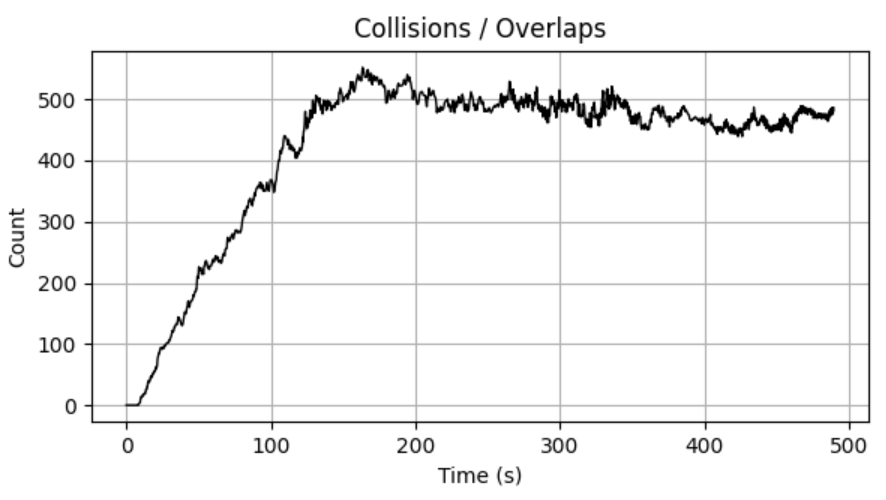
\includegraphics[width=0.8\columnwidth]{images/collisions_overlaps.png}
    \caption{Number of collisions or overlaps accumulated over time.}
    \label{fig:collisions}
\end{figure}

\FloatBarrier

\subsection{\textbf{Travel Time and Distance}}

Travel efficiency is evaluated using distributions of individual agent travel
times. These distributions expose variability in evacuation efficiency across
agents.

Path efficiency is quantified using the detour index. For each agent $i$, the
detour index is defined as
\begin{equation}
    D_i = \frac{L_i}{L_i^{\text{straight}}},
\end{equation}
where $L_i$ is the total distance traveled by the agent and
$L_i^{\text{straight}}$ is the straight-line distance from the spawn location
to the assigned exit. The reported detour metric is the mean value over all
agents.

\begin{figure}[htbp]
    \centering
    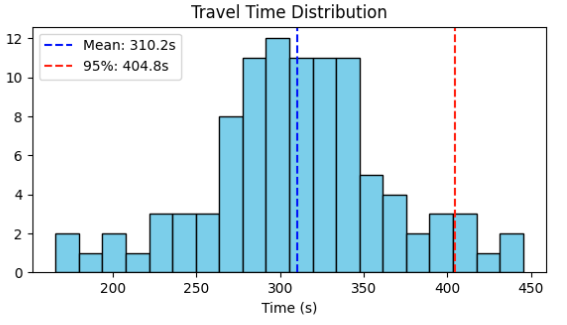
\includegraphics[width=0.8\columnwidth]{images/tim_travel_dist.png}
    \caption{Distribution of individual agent travel times from entry to exit.}
    \label{fig:travel_time_dist}
\end{figure}

\FloatBarrier

\section{Results and Analysis}

This section presents the experimental results obtained from multiple crowd
simulation scenarios and analyzes the observed behaviors using the evaluation
metrics defined earlier. The goal is to assess both evacuation efficiency and
crowd dynamics under varying conditions.

\subsection{\textbf{Quantitative Results}}

Quantitative results are summarized using tables that report evacuation time,
average throughput, peak crowd density, and simulation performance across
different scenarios. As expected, evacuation time increases with the number of
agents, while throughput initially rises and then stabilizes as exits reach
capacity. Peak density values are consistently observed near exits and narrow
corridors, confirming the presence of bottlenecks in high-density scenarios.
Overall, the results demonstrate stable and consistent trends across repeated
simulation runs.

(Place Table I here: Summary of evacuation time, peak density, and throughput for all scenarios.)

\subsection{\textbf{Graph and Plots}}

Graphs are used to better understand how crowd behavior evolves over time.
Cumulative evacuation curves show that low-density scenarios exhibit smooth,
near-linear evacuation, whereas high-density cases display slower and
non-linear progression due to congestion. Density heatmaps visually highlight
regions where crowding persists, while flow-rate plots reveal short-term
fluctuations in exit usage. Performance plots indicate that the simulation
maintains interactive frame rates for moderate crowd sizes, with gradual
degradation as agent count increases.

\subsection{\textbf{Scenario-Wise Performance}}

Scenario-wise analysis shows clear differences in crowd behavior depending on
layout and population size. In simple layouts with wide exits, agents
distribute evenly and evacuate efficiently with minimal congestion. More
complex layouts, such as those with narrow exits or sharp turns, result in
localized density buildup and reduced throughput. High-population scenarios
amplify these effects, leading to longer evacuation times and visible queuing
behavior. Despite these challenges, the simulation remains stable and produces
realistic emergent patterns across all tested scenarios.

\section{Visualization and Observation}

\begin{figure}[htbp]
    \centering
    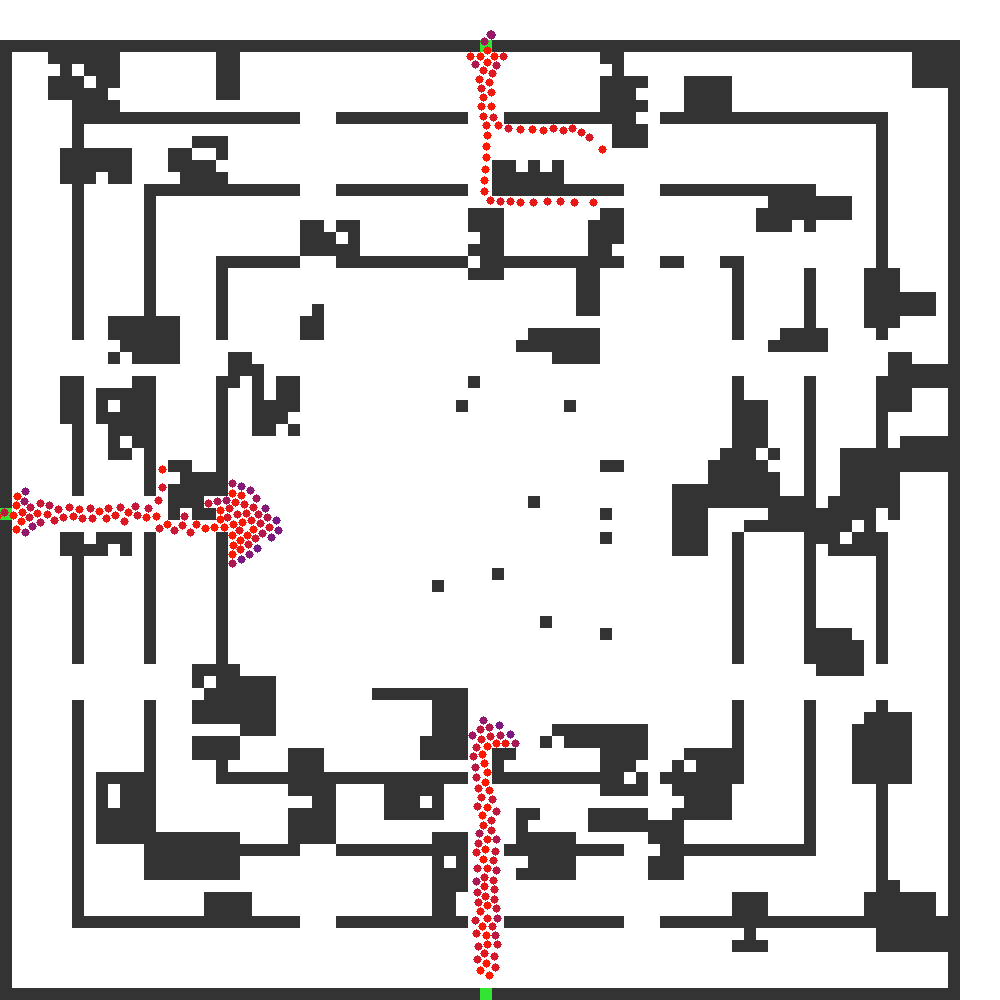
\includegraphics[width=0.48\columnwidth]{images/snapshot.png}
    \caption{Simulation snapshot showing agent distribution and movement patterns at a representative time step during evacuation. The snapshot illustrates spatial organization, congestion regions, and overall crowd flow behavior.}
    \label{fig:simulation_snapshot}
\end{figure}

\begin{figure}[htbp]
    \centering
    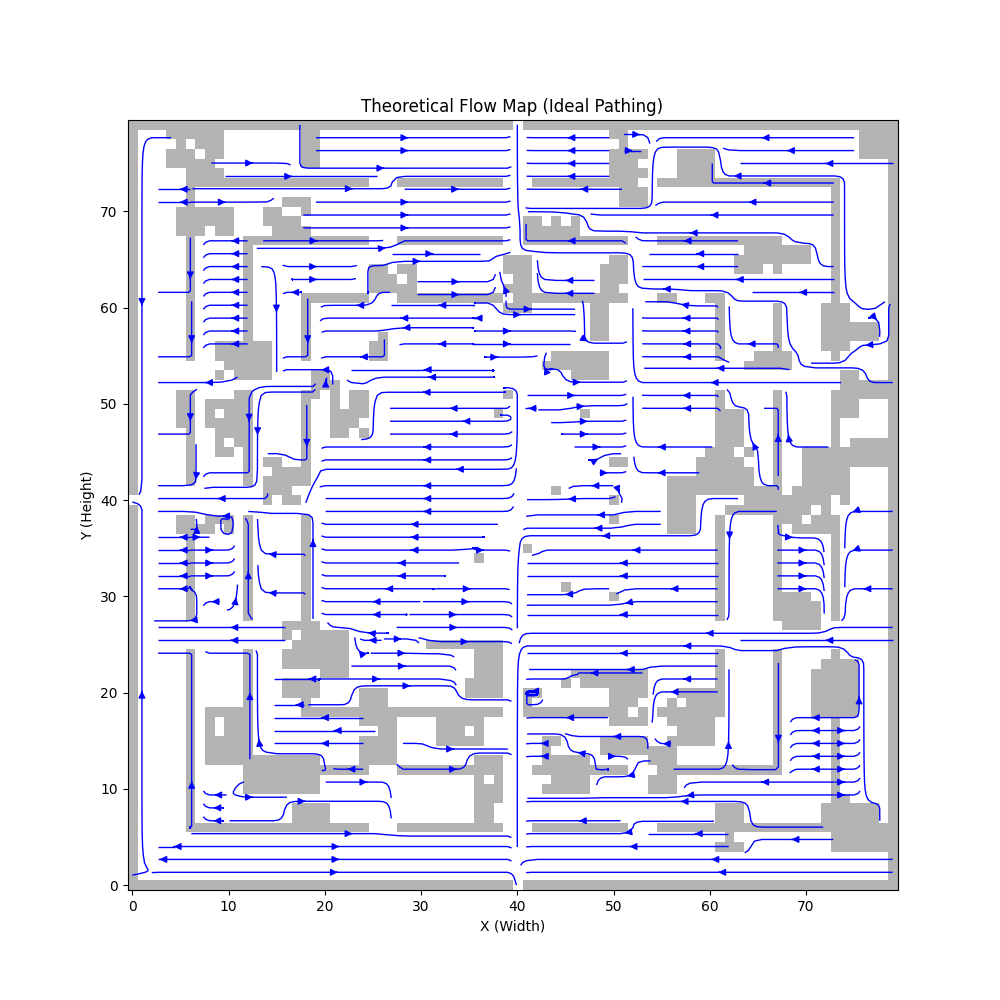
\includegraphics[width=0.48\columnwidth]{images/heatmap_theoretical_flow.png}
    \hfill
    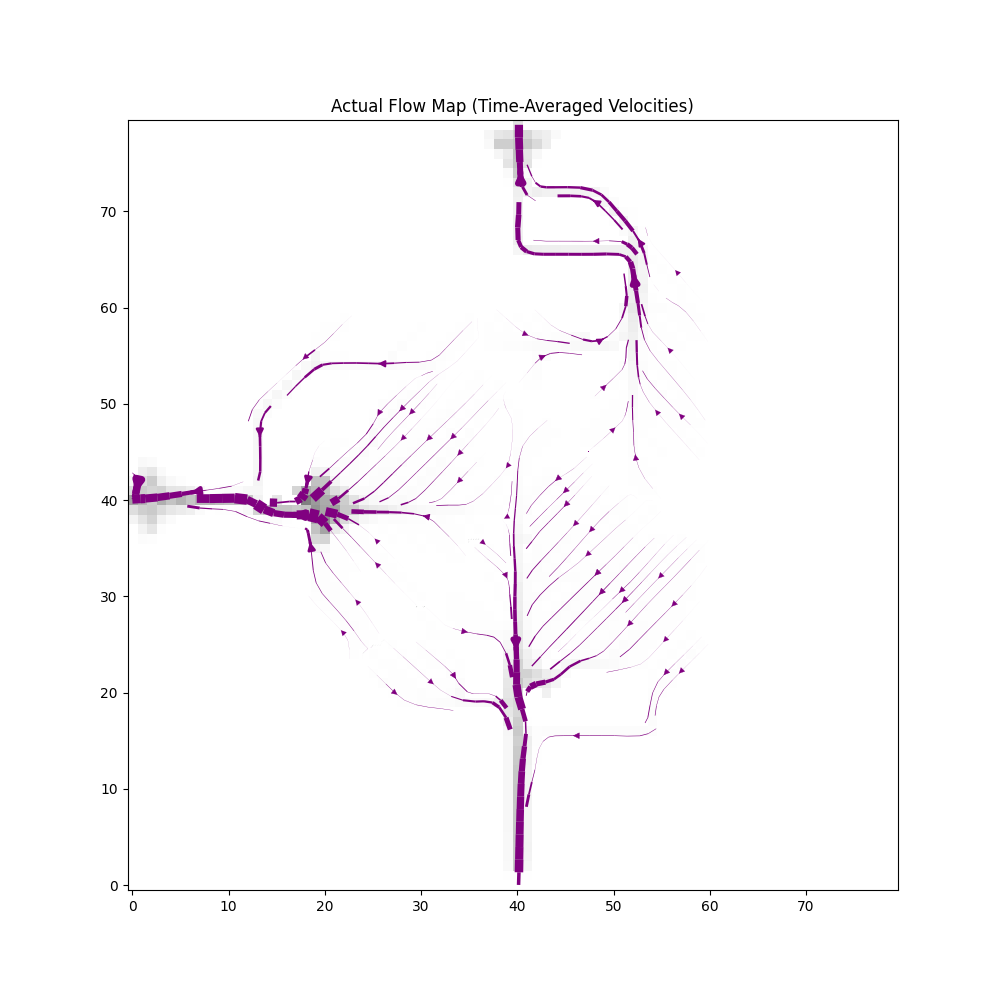
\includegraphics[width=0.48\columnwidth]{images/heatmap_actual_flow.png}
    \caption{Behavioral flow comparison. (Left) Theoretical flow heatmap representing idealized pedestrian movement based on shortest paths and uniform behavior assumptions. (Right) Actual flow heatmap obtained from the simulation, reflecting emergent crowd behavior, congestion effects, and local interactions.}
    \label{fig:behavioral_flow_comparison}
\end{figure}

\section{Limitations}

While the proposed crowd simulation framework is effective for modeling
pedestrian movement in indoor environments, it has several limitations that
should be acknowledged. These limitations arise from design choices made to
keep the system simple, interpretable, and computationally efficient.

\subsection{\textbf{Model Constrains}}

The model operates in a two-dimensional space and represents the environment
using static floor-plan images. As a result, vertical movement (such as stairs
or multiple floors) and dynamic environmental changes are not considered.
Agents are modeled with simplified physical and behavioral characteristics,
which may not capture complex human factors such as panic, decision-making
under stress, or social group dynamics.

\subsection{\textbf{Assumptions}}

Several assumptions are made to simplify the simulation. Agents are assumed to
have similar physical abilities and follow rational, goal-oriented behavior
toward exits. The environment is treated as static, with exits always available
and clearly defined. Interactions with furniture, signage, or dynamically
changing obstacles are not explicitly modeled. These assumptions help maintain
clarity and stability but may limit realism in certain real-world scenarios.

\subsection{\textbf{Scalability Issues}}

Although the framework performs efficiently for moderate crowd sizes,
performance can degrade as the number of agents increases significantly. Local
collision-avoidance computations become more expensive at high densities, which
may reduce simulation speed and visualization frame rates. While suitable for
interactive analysis and academic experiments, very large-scale scenarios may
require further optimization or parallelization to maintain real-time
performance.

\section{Future Work}

\subsection{\textbf{Extensions}}

Future work can extend the system to support multi-floor and three-dimensional
environments by incorporating staircases, elevators, and vertical connectivity
between levels. Agent heterogeneity can also be introduced by varying walking
speeds, physical dimensions, and behavioral preferences to better reflect real
populations. Additionally, support for dynamic environments—such as temporary
obstacles, blocked exits, or changing signage—would allow simulation of more
realistic emergency and event-based scenarios.

\subsection{\textbf{Real-world Deployment Possibilities}}

With further validation, the framework could be applied in real-world settings
such as evacuation planning for academic buildings, shopping malls, hospitals,
and transportation hubs. Integration with building information models (BIM) or
live sensor data (e.g., CCTV, occupancy counters) could enable near real-time
monitoring and decision support. Such deployments would help planners and
safety personnel evaluate design choices, test evacuation strategies, and
improve crowd management policies before implementation.

\subsection{\textbf{Advanced Modeling Ideas}}

More advanced behavior models could be incorporated to capture psychological
and social factors, including panic propagation, group movement, and
leader–follower dynamics. Learning-based components may be explored to
calibrate agent behavior using real trajectory data or to adapt navigation
strategies over time. Hybrid approaches that combine the current rule-based
framework with data-driven models could improve realism while preserving
interpretability and computational efficiency.

\section{Conclusion}

In this work, a modular and image-driven crowd simulation framework was
developed that converts architectural floor-plan images into walkable
representations, computes global navigation cues using distance fields, and
combines these with local avoidance to produce realistic pedestrian behaviors.
This approach enables simulation of evacuation dynamics, congestion patterns,
and throughput under varied scenarios without relying on detailed CAD models or
extensive data calibration. The paper demonstrated how the preprocessing
pipeline, agent behavior model, and evaluation metrics work together to provide
meaningful insights into evacuation performance across different layout
configurations and crowd densities. Key outcomes include clear trends in
evacuation times and throughput, visualization of high-density regions and
bottlenecks, and scalable performance for moderate agent counts, suggesting
that the system is suitable for academic experimentation and early design
analysis. While limitations exist—such as simplified agent characteristics and
static environments—the framework makes a practical contribution by balancing
interpretability, computational efficiency, and emergent crowd phenomena. These
results support the value of lightweight, image-based simulation tools in
facility planning and safety evaluation, and encourage further extensions
toward real-world deployments and richer behavioral models.

\begin{thebibliography}{00}

    \bibitem{helbing1995social}
    D. Helbing and P. Molnár, ``Social force model for pedestrian dynamics,''
    \emph{Physical Review E}, vol. 51, no. 5, pp. 4282--4286, 1995.

    \bibitem{helbing2000social}
    D. Helbing, I. Farkas, and T. Vicsek, ``Simulating dynamical features of escape
    panic,'' \emph{Nature}, vol. 407, no. 6803, pp. 487--490, 2000.

    \bibitem{van2008reciprocal}
    J. van den Berg, M. Lin, and D. Manocha, ``Reciprocal velocity obstacles for
    real-time multi-agent navigation,'' in \emph{Proc. IEEE Int. Conf. Robotics and
        Automation}, 2008, pp. 1928--1935.

    \bibitem{berg2011reciprocal}
    J. van den Berg, S. Guy, M. Lin, and D. Manocha, ``Reciprocal n-body collision
    avoidance,'' in \emph{Robotics Research}, Springer, 2011, pp. 3--19.

    \bibitem{pan2016crowd}
    X. Pan, M. Han, K. Dauber, and K. H. Law, ``A multi-agent based framework for the
    simulation of human and social behaviors during emergency evacuations,''
    \emph{AI \& Society}, vol. 22, no. 2, pp. 113--132, 2006.

    \bibitem{alahi2016social}
    A. Alahi \emph{et al.}, ``Social LSTM:\@ Human trajectory prediction in crowded
    spaces,'' in \emph{Proc. IEEE Conf. Computer Vision and Pattern Recognition},
    2016, pp. 961--971.

    \bibitem{sethian1996fast}
    J. A. Sethian, ``A fast marching level set method for monotonically advancing
    fronts,'' \emph{Proc. Natl. Acad. Sci.}, vol. 93, no. 4, pp. 1591--1595, 1996.

    \bibitem{hoogendoorn2004pedestrian}
    S. P. Hoogendoorn and P. H. L. Bovy, ``Pedestrian route-choice and activity
    scheduling theory and models,'' \emph{Transportation Research Part B},
    vol. 38, no. 2, pp. 169--190, 2004.

    \bibitem{seyfried2005fundamental}
    A. Seyfried, B. Steffen, and T. Lippert, ``Fundamental diagram of pedestrian
    movement revisited,'' \emph{Journal of Statistical Mechanics}, vol. 2005,
    no. 10, P10002, 2005.

    \bibitem{chen2018floorplan}
    C. Chen, A. Saxena, and J. Xiong, ``Floorplan analysis for indoor navigation
    using deep learning,'' in \emph{Proc. IEEE Int. Conf. Pattern Recognition},
    2018, pp. 135--140.

    \bibitem{battaglia2021path}
    P. Battaglia, J. Hamrick, and V. Bapst, ``Relational inductive biases, deep
    learning, and graph networks,'' \emph{arXiv preprint arXiv:1806.01261}, 2018.

\end{thebibliography}

\vspace{12pt}

\end{document}
